\section{Paper 2: Vector Quantized VAE (VQ-VAE)}
Title:  \textit{Neural Discrete Representation Learning} \cite{oord_neural_2018}.
\\



Main points: 
\begin{itemize}
    \item Avoiding Posterior Collapse
    \item Discrete Latent
    \item With the right prior, generates speech/audio well  % TODO: elaborat
    \item Language Learning through raw speech
    \item Speaker Conversion
\end{itemize}


The main point of the VQ-VAE lies in that it uses a discrete (i.e. \textit{categorical}) embedding space as its latent space. 


\subsection{Model Components and Architecture}
The model is described in \cref{fig:vqvae-arch}.
What's very important to realize is that \textbf{the VQ-VAE is deterministic, not stochastic!}

\subsection{Discrete Latent Embedding Space}
The VQ VAE uses a \(D\)-dimensional latent space with \(K\) embedding vectors.
This means that the latent space \textbf{does not sample from a latent space} (so it's not a real VAE) but instead \textbf{does a nearest-neighbor embedding lookup}. 
We define the embedding vectors as 
\[
  e_i \in \mathbb{R}^D, i \in \{1 .. K\}, \therefore e \in \mathbb{R}^{K \times D}
\]

\begin{figure}[ht]
    \begin{small}
        \begin{center}
            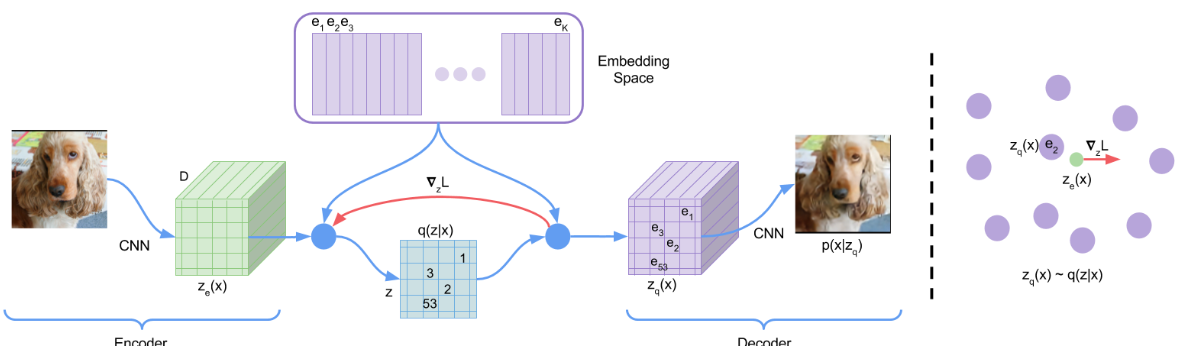
\includegraphics[width=0.95\textwidth]{figures/vqvae-arch}
        \end{center}
        \caption{VQ-VAE Architecture. 
        Right: Embedding space. 
        Left: Overall Architecture. 
        Note that the CNN works as a down/upsampling CNN, so as to avoid identity operations all the way through. 
        }
        \label{fig:vqvae-arch}
    \end{small}
\end{figure}

\subsection{Loss function}

The loss function \cref{eq:vqvae-loss} is composed of 3 parts, here covered in detail:

\begin{equation}
    L = 
    \log p(x| z_q(x)) + 
    || \mathrm{sg}[z_e (x) ] - e ||_2^2 + 
    || z_e (x)  - \mathrm{sg}[e] ||_2^2
    \label{eq:vqvae-loss}
\end{equation}

We denote \(z_e(x)\) as the \textbf{encoder output} and \(z_q(x)\) as the \textbf{quantized encoding.} 
We also use \(\mathrm{sg}\) to denote the stopgradient operator (identity function forward but 0 partial derivatives).

\paragraph{Reconstruction Loss}
\[
    \log p(x| z_q(x)) +     
\]
This refers to the probability of the data \(x\) given the embedding \(z_q(x)\).

The reconstruction loss is optimized by the \textbf{encoder} and \textbf{decoder}.

\paragraph{Embedding Loss}
\[
    || \mathrm{sg}[z_e (x) ] - e ||_2^2 
\]

The embedding loss quantifies \textit{how far away from the samples the embeddings are.}
This loss comes from Vector Quantization (VQ), a dictionary learning algorithm. 
The VQ objective seen here moves the \textit{discretized} embedding vectors \(e_i \in \mathbb{R}^D\) towards the \textit{continuous encoder outputs} \(z_e(x)\).
This means that the model is able to learn embeddings and update them at need. 

The embedding loss is optimized by the \textbf{embedding}.

\paragraph{Commitment Loss}
\[
    || z_e (x)  - \mathrm{sg}[e] ||_2^2
\]
The commitment loss quantifies \textit{how far away from the embeddings a sample is.}
The embedding space is dimensionless in volume, and therefore the output of the encoder can grow arbitrarily large, while embeddings can't keep up. 
This equates to the encoder seeing an out-of-distribution sample and encoding it as very far away from the latent space embeddings. 

The commitment loss is optimized by the \textbf{encoder}.



\subsection{Experiments and Results}

\subsubsection{Images}
Downsampling from \(128 \times 128 \times 3 \) to a \( 32 \times 32 \times 1 \) discretized latent space on the ImageNet ( \(128 \times 128 \times 3\) ) dataset.

For images, the encoder/decoder is the PixelCNN. 



\subsubsection{Audio}
For audio, the VQ-VAE is trained on the VCTK dataset, which has 109 different speakers. 
The encoder is \textbf{6 strided convolutions with stride 2 and window-size 4}, corresponding to a downsampling of 64x. 
The latent space is a single 512-dimensional discretized space. 
In addition to the latent space, the decoder is conditioned on a 1-hot speaker embedding. 

\paragraph{Results}
The VQ-VAE manages to learn to interchange speakers very well. To cite the paper:

\begin{displayquote}
    This means that the VQ-VAE has, without any form of linguistic supervision, 
    learned a high-level abstract space that is invariant to low-level features and only encodes the content of the speech.
\end{displayquote}


The authors also ran an experiment where they mapped a 128-dimensional discrete latent space to 41 phonemes. 
Using this simple mapping they found the accuracy to be \(49.3\%\), without further mappings. 

